\documentclass[main.tex]{subfiles}

\begin{document}
\pagebreak
\chapter[XBee Configuration]{XBee Configuration}

\begin{center}
	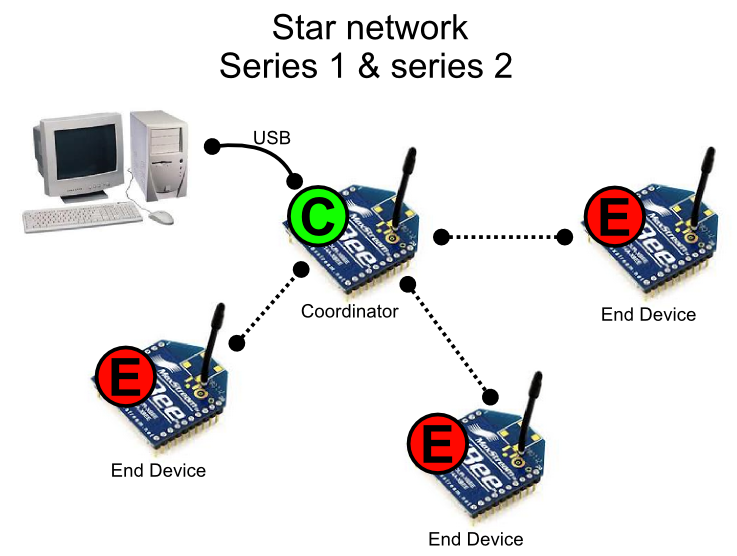
\includegraphics[scale = .447]{Images/star.png}
\end{center}

Set the baudrate to 115200 of every Xbee module.
Baudrate is the speed of communication between XBee and connected device.

\noindent
\includegraphics[scale=1]{Images/baudrate.png}
\section{API mode}
Set API Enable for every xbee module


\includegraphics[scale=1]{Images/apienb.png}

In API mode data, is sent from one XBee to another in packets which ensures that the data is not corrupted and is legal. It also enable point to point communication of two Xbee devices without disturbing other Xbee on the channel.
Each XBee on the channel has a unique id which is embedded in the packet so the XBee with the id will decode the packet.
\subsection{Coordinator}

\includegraphics[scale=1]{Images/corenb.png}

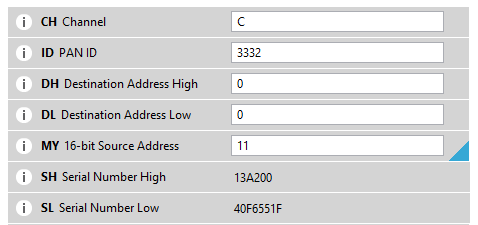
\includegraphics[scale=1]{Images/apicord.png}

DH-0

DL-0
 
My id-11 \#unique id for each xbee

API mode :Enabled
\subsection{End device}


\includegraphics[scale=1]{Images/endenb.png}

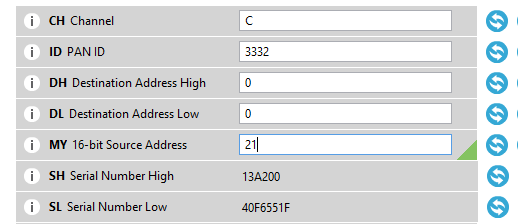
\includegraphics[scale=1]{Images/apiend.png}

DH-0
DL=0

My id:21 \#unique id for every end xbee. For example(22,23,24 etc..)

API mode : Enabled
\pagebreak
\section{AT mode}
Set API to Disable for every module

\noindent
\includegraphics[scale=1]{Images/apidisable.png}

In AT mode data is send character by character to every XBee or only a pre-defined XBee based on the destination address.
Chances of data corruption is higher. 

Sending all the data to each and every XBee is tough to use in swarm robots as the microcontroller has to be able to receive and decode all the data which is sent to all the XBees. 
Microcontroller will need to have good data handling capabilities to handle so much data.
AT mode is good for point to point communication.

\pagebreak
\subsection{Coordinator}

\includegraphics[scale=1]{Images/corenb.png}

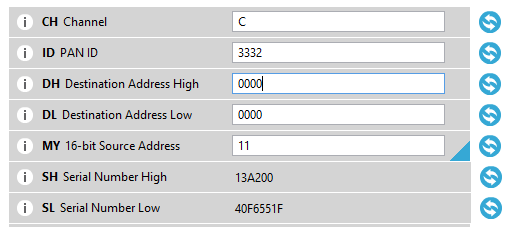
\includegraphics[scale=1]{Images/atcord.png}

\noindent\textbf{Broadcast Mode}\\
DH-0000\\ 
DL-0000 \\
My id: ``any positive int 16 bit"\\

\noindent\textbf{Point to Point}
DH-High serial number of end module\\ 
DL-Low serial number of end module Or My id of end module\\
My id: ``any positive int 16 bit"

\pagebreak
\subsection{End device}

\includegraphics[scale=1]{Images/endenb.png}

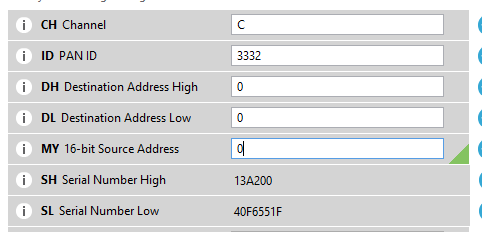
\includegraphics[scale=1]{Images/atend.png}

\noindent\textbf{Broadcast Mode}
DH-0000\\ 
DL-0000 \\
My id: 0000\\

\noindent\textbf{Point to Point}
DH-0000\\ 
DL-0000\\
My id: "any positive int 16 bit"

\end{document}